\chapter{Graphical Neural Network Prototyping}
In the last chapter we visualize the steps from data processing, over the model development and to final evaluation from the previous chapters. This visualization should add to a better understanding of the presented data and to enable quick prototyping.

First we will look at the general software structure to understand the source code we are going to develop. This is important to build a clean framework that allows an easy exchange of modules, functions and code. \newline
Once the code structure is established, we will present a tutorial for the workflow of the developed GUI. The workflow will follow the past chapters starting with the data representation and feature selection, going through the \ac{nn} development and finish with the evaluation of the model as well as the established baseline.

	\section{Software Structure}
	The presented software structure here divides graphics and data handling into two explicitly separated parts. The graphics part will be build with the Python framework of Qt \cite{qt-web} and the data handling part mostly with Tensorflow \cite{tf-web}.
	
	In figure \ref{f:gui_source_flow} the rough intention of the work and design flow is shown. It can be seen that we start with the user input via events on the graphical elements. These graphical elements will forward the entered data to the data-handling module. As said, the data-handling module contains everything to transform the data and handle the given \ac{nn}. Once all the data is processed, the results are written back to the graphical elements to inform the user. \newline
	The graphical elements are stored in the \enquote{SubWindow.py} and the data-handling in the \enquote{SubModule.py}. We will investigate both modules further in the next two sections.
	
	\begin{figure}[htb]
	\centering
	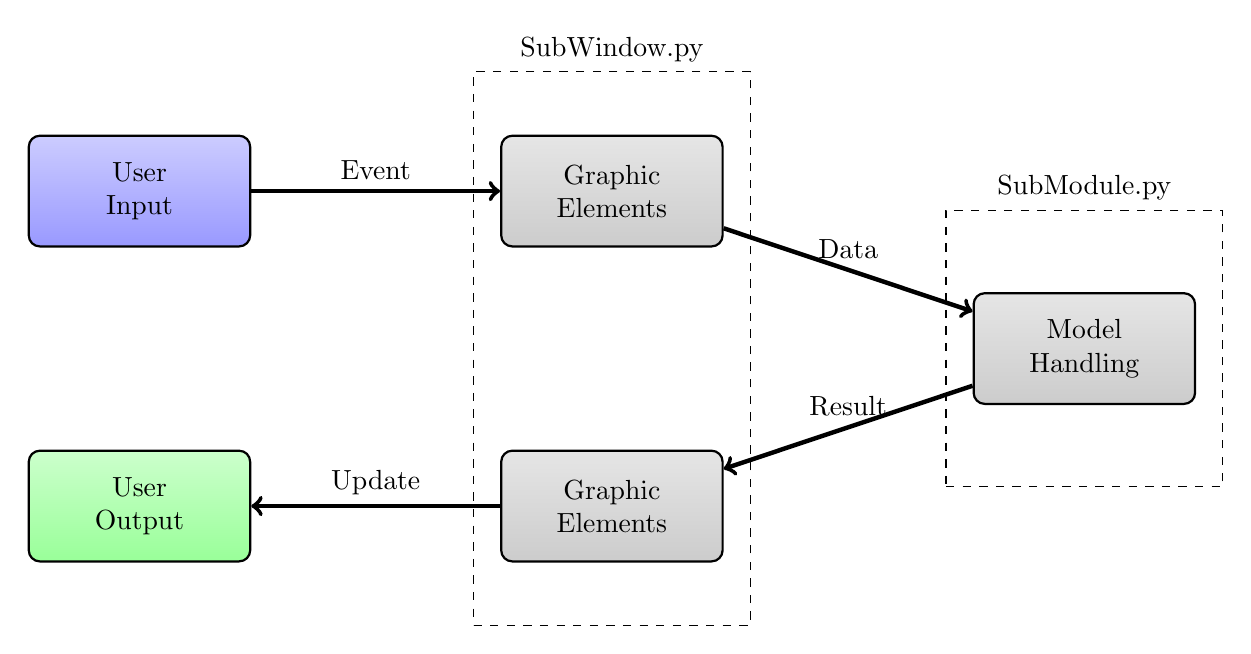
\begin{tikzpicture}[
	input/.style={
		rectangle,
		draw=black,
		thick,
		align=center,
		rounded corners,
		top color=blue!20,
		bottom color=blue!40,
		minimum height=4em,
		minimum width=8em
	},
	neuron/.style={
		rectangle,
		draw=black,
		thick,
		align=center,
		rounded corners,
		top color=gray!20,
		bottom color=gray!40,
		minimum height=4em,
		minimum width=8em
	},
	output/.style={
		rectangle,
		draw=black,
		thick,
		align=center,
		rounded corners,
		top color=green!20,
		bottom color=green!40,
		minimum height=4em,
		minimum width=8em
	},
]

\node[input] (ui) at (-6, 2) {User \\ Input};
\node[neuron] (graphic1) at (0, 2) {Graphic \\ Elements};
\node[neuron] (model) at (6, 0) {Model \\ Handling};

\node[neuron] (graphic2) at (0, -2) {Graphic \\ Elements};
\node[output] (uo) at (-6, -2) {User \\ Output};

\draw[ultra thick, ->] (ui) -- node [above] {Event} (graphic1);
\draw[ultra thick, ->] (graphic1) -- node [above] {Data} (model);
\draw[ultra thick, ->] (model) -- node [above] {Result} (graphic2);
\draw[ultra thick, ->] (graphic2) -- node [above] {Update} (uo);

\node[rectangle, dashed, draw=black, align=center, minimum height=20em, minimum width=10em] 
(SubWindow) at (0, 0) {};
\node[above] at (SubWindow.north) {SubWindow.py};

\node[rectangle, dashed, draw=black, align=center, minimum height=10em, minimum width=10em] 
(SubModule) at (6, 0) {};
\node[above] at (SubModule.north) {SubModule.py};

\end{tikzpicture}
	\caption{Action flow of the GUI, starting with the user input managed via graphical elements that push the data to the data-handling module, which then updates the graphical elements to notify the user.}
	\label{f:gui_source_flow}
	\end{figure}	
	
		\subsection{Graphics Handling}
		As mentioned above, the graphics are done in \enquote{SubWindow.py} with the help of the Qt framework.	In figure \ref{f:subwindow_py} an outline of the file is shown with the three separate tabs containing different graphical elements. 
		
		The data tab is the first one and it will represent all the data in a plot. Additionally it features radio buttons to set features according to their categories of deterministic, aleotric, prediction or none (if not used). At last a checkbox determining whether the feature shall be one-hot-encoded is implemented. Also already concerning the network, the data tab should allow setting starting points for the subsets of validation and test data. 
		
		The network tab should contain a texteditor for writing and defining the \ac{nn} layers. To compile, train, evaluate and store the network, respective push buttons will be needed and connected to the data-handling module. For setting the various hyperparameters a numerical dial will be used with pre-defined boundaries. The numerical evaluation result will be displayed at the top.
		
		At last the prediction tab will contain a plot to show a prediction of 24 hours together with the uncertainty and the ground truth data. 

		\begin{figure}[htb]
		\centering
		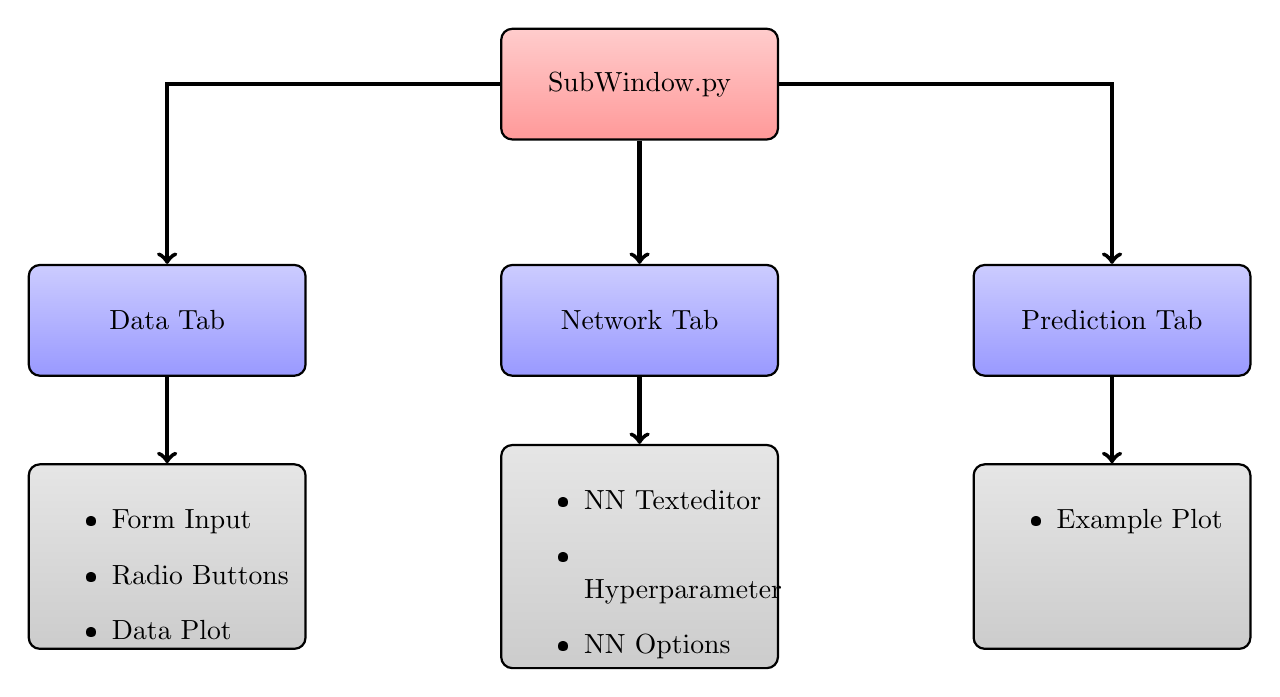
\begin{tikzpicture}[
	top/.style={
		rectangle,
		draw=black,
		thick,
		align=center,
		rounded corners,
		top color=red!20,
		bottom color=red!40,
		minimum height=4em,
		minimum width=10em
	},
	mid/.style={
		rectangle,
		draw=black,
		thick,
		align=center,
		rounded corners,
		top color=blue!20,
		bottom color=blue!40,
		minimum height=4em,
		minimum width=10em
	},
	bottom/.style={
		rectangle,
		draw=black,
		thick,
		align=center,
		text width=9em,
		rounded corners,
		top color=gray!20,
		bottom color=gray!40,
		minimum height=4em,
		minimum width=10em
	},
]

\node[top] (top) at (0, 3) {SubWindow.py};

\node[mid] (mid_data) at (-6, 0) {Data Tab};
\node[mid] (mid_net) at (0, 0) {Network Tab};
\node[mid] (mid_pred) at (6, 0) {Prediction Tab};

\node[bottom] (bottom_data) at (-6, -3) {\begin{itemize} 
	\item Form Input
	\item Radio Buttons
	\item Data Plot
\end{itemize}};

\node[bottom] (bottom_net) at (0, -3) {\begin{itemize} 
	\item NN Texteditor	
	\item Hyperparameter
	\item NN Options
\end{itemize}};

\node[bottom] (bottom_pred) at (6, -3) {\begin{itemize} 
	\item Example Plot
	\item[] 
	\item[]
\end{itemize}};

\draw[ultra thick,->, to path={-| (\tikztotarget)}] (top) edge (mid_data);
\draw[ultra thick,->] (top) edge (mid_net);
\draw[ultra thick,->, to path={-| (\tikztotarget)}] (top) edge (mid_pred);

\draw[ultra thick,->] (mid_data) -- (bottom_data);
\draw[ultra thick,->] (mid_net) -- (bottom_net);
\draw[ultra thick,->] (mid_pred) -- (bottom_pred);

\end{tikzpicture}
		\caption{Outline of the SubWindow with the three tabs containing various graphical elements needed for user interaction.}
		\label{f:subwindow_py}
		\end{figure}
			
		\subsection{Data Handling}
		The data-handling module is embedded in the \enquote{SubModule.py}, outlined in figure \ref{f:submodule_py}. It takes data entered in the UI via the \enquote{SubWindow.py} interface, performs computations and hands the result back. Here lies the implementation of the handling of the dataset (e.g. a set of reaction wheel parameters) and the execution of the \ac{nn}. The structure follows the one of the graphics handling above with the three different tabs.
		
		In the data tab, the dataset is read and divided in training, validation and test. The data is sorted according to the feature definitions. First comes the label or prediction feature, after that follow the aleatoric features and at last the deterministic ones. A Tensorflow function is then used to create trainable datasets. They are shuffled and batched in a size of 32.
		
		The network tab contains hyperparameters setting, the compilation, training and evaluation, which are mostly implemented as simple set-methods or wrapper functions for Tensorflow. The network definition entered in the graphical texteditor is implemented between network inputs and outputs and executed in form of a Python subprocess. \newline
		The evaluation of the network also contains the implemented baseline discussed above.
		
		At last the prediction tab randomly selects an example from the test set, feeds it through the trained network and returns mean as well as standard-deviation.

		\begin{figure}[htb]
		\centering
		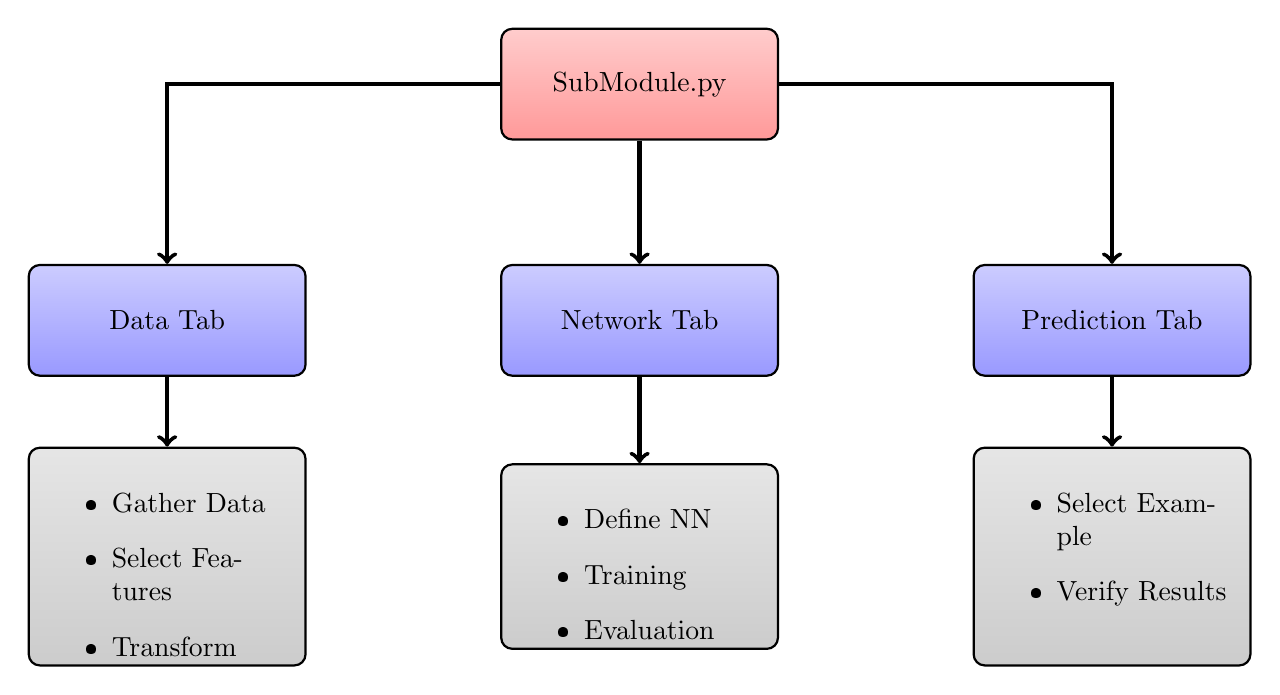
\begin{tikzpicture}[
	top/.style={
		rectangle,
		draw=black,
		thick,
		align=center,
		rounded corners,
		top color=red!20,
		bottom color=red!40,
		minimum height=4em,
		minimum width=10em
	},
	mid/.style={
		rectangle,
		draw=black,
		thick,
		align=center,
		rounded corners,
		top color=blue!20,
		bottom color=blue!40,
		minimum height=4em,
		minimum width=10em
	},
	bottom/.style={
		rectangle,
		draw=black,
		thick,
		align=center,
		text width=9em,
		rounded corners,
		top color=gray!20,
		bottom color=gray!40,
		minimum height=4em,
		minimum width=10em
	},
]

\node[top] (top) at (0, 3) {SubModule.py};

\node[mid] (mid_data) at (-6, 0) {Data Tab};
\node[mid] (mid_net) at (0, 0) {Network Tab};
\node[mid] (mid_pred) at (6, 0) {Prediction Tab};

\node[bottom] (bottom_data) at (-6, -3) {\begin{itemize} 
	\item Gather Data	
	\item Select Features 
	\item Transform
\end{itemize}};

\node[bottom] (bottom_net) at (0, -3) {\begin{itemize} 
	\item Define NN	
	\item Training
	\item Evaluation
\end{itemize}};

\node[bottom] (bottom_pred) at (6, -3) {\begin{itemize} 
	\item Select Example
	\item Verify Results 
	\item[]
\end{itemize}};

\draw[ultra thick,->, to path={-| (\tikztotarget)}] (top) edge (mid_data);
\draw[ultra thick,->] (top) edge (mid_net);
\draw[ultra thick,->, to path={-| (\tikztotarget)}] (top) edge (mid_pred);

\draw[ultra thick,->] (mid_data) -- (bottom_data);
\draw[ultra thick,->] (mid_net) -- (bottom_net);
\draw[ultra thick,->] (mid_pred) -- (bottom_pred);

\end{tikzpicture}
		\caption{Outline of the SubModule with the three tabs containing the underlying calculation for the user input / output.}
		\label{f:submodule_py}
		\end{figure}	
		
	\section{Workflow}
	Now that we have the structure of the GUI and wrote all the underlying code, we can show how to work with the GUI. The workflow is again oriented on the whole structure of this thesis.
	
	We first start with the data tab where we load the dataset, prepared according to chapter \ref{c:datamining}. This means we have cleaned and pre-analysed our data and we already decided which columns to hot-encode and therefore converted them to integers. The value range of the dataset doesn't need to be adapted. \newline
	In the second tab the model is generated and the hyperparameters are adjusted with respect to the assumptions and knowledge from chapter \ref{c:prediction}. \newline
	At last follows the prediction tab, where we can switch through examples, which are then plotted for our visualization.
	
		\subsection{Data Tab}
		The data tab refers to the data mining in chapter \ref{c:datamining}. In figure \ref{f:gui_data_tab} we can see a screenshot of the data tab. On top we have various options and on the bottom a full plot of all our data, normalized to a range of 0 to 1.
		
		The options on the top left concern the whole dataset. Here we can toggle an \enquote{FFT} box to see the frequency plot of our dataset and quickly check for any periodic appearances. Below we can choose to smoothen our dataset to attenuate high frequencies. Further below we can set the sample point where the validation set and the test set start, by default they are set at 80\% and 90\% of the whole dataset. \newline
		On the right the features are presented. They can be put in the 3 categories (deterministic, aleatoric and prediction) or turned off. Additionally a checkbox at the very bottom allows to select a feature for one-hot-encoding. Care must be taken to correctly select the features in order to get good results from the \ac{nn}. 
		
		At the bottom all selected features are plotted in a value range of 0 to 1. By default all data is visible, but the plot element allows for magnification on areas of interest.
		
		\begin{figure}[htb]
		\centering
		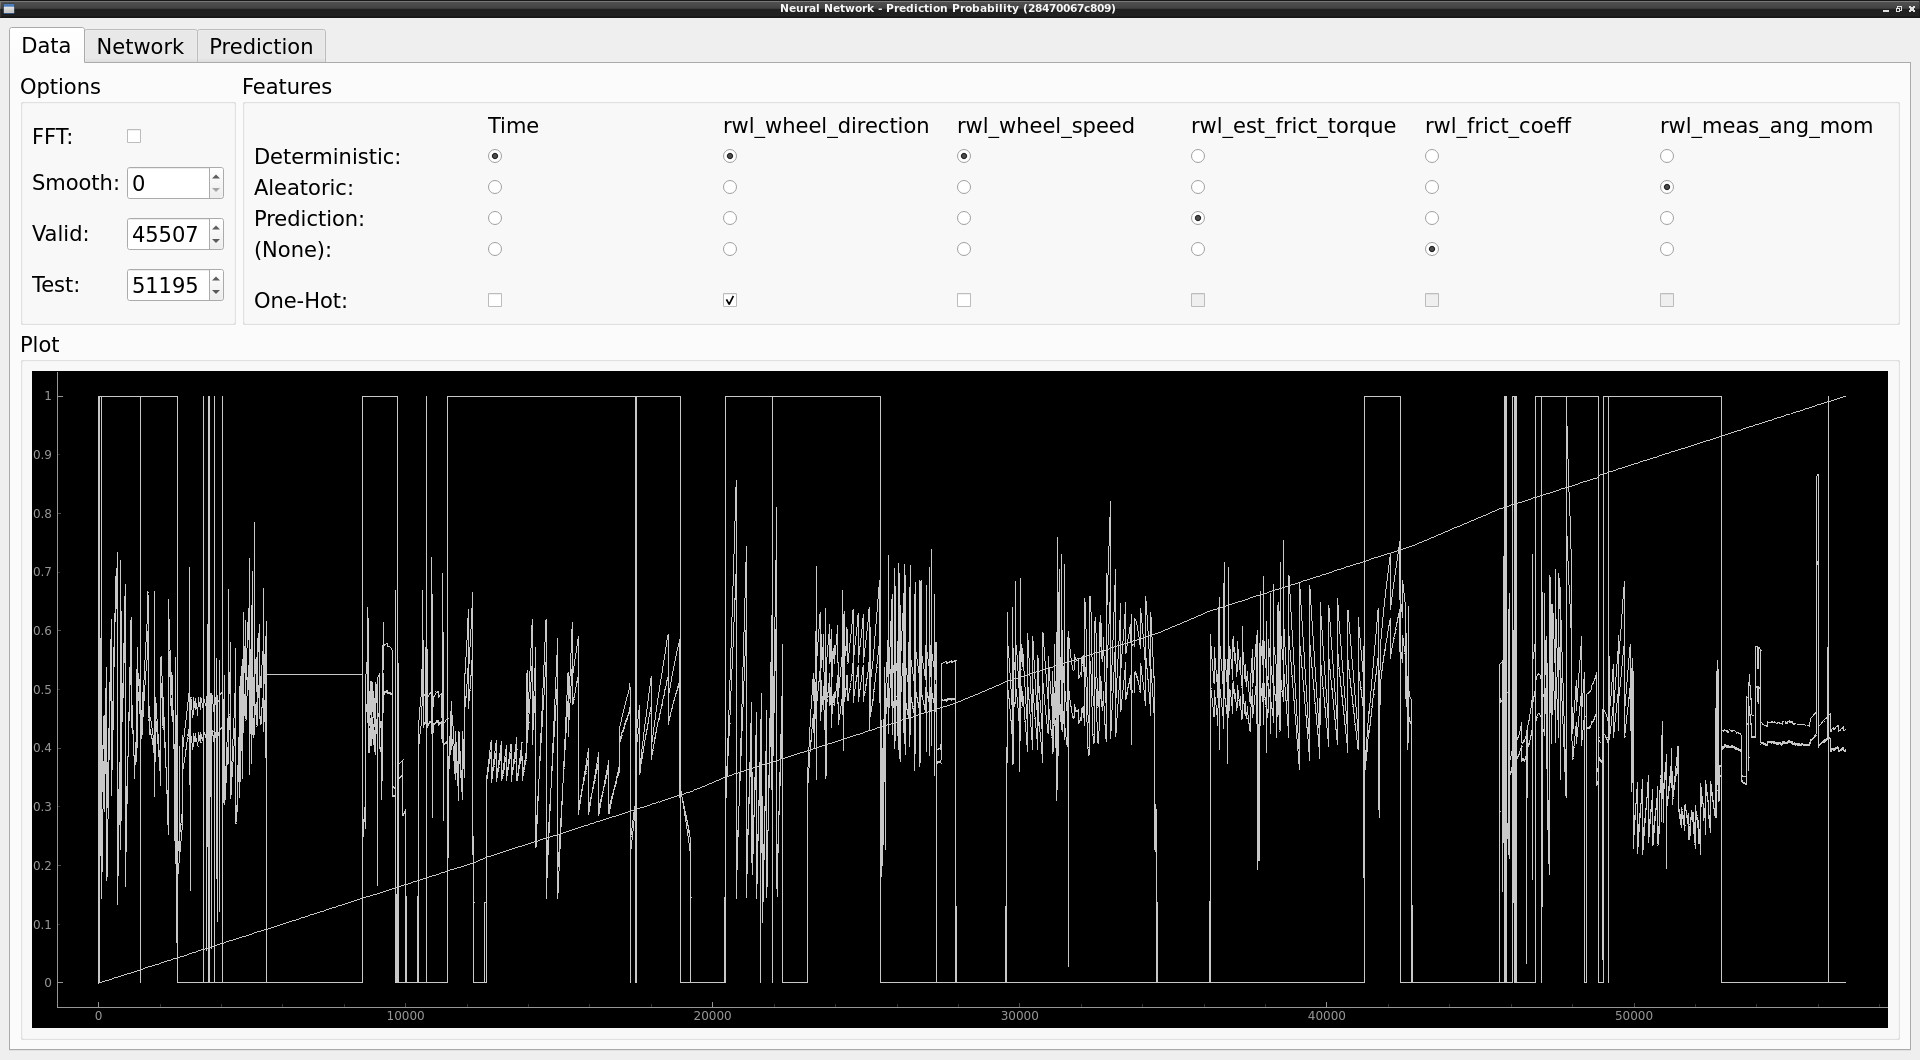
\includegraphics[width=0.9\textwidth]{./4_GUI/gui_data_tab.jpg}
		\caption{Screenshot of the data tab of the GUI. Various selectable options regarding the dataset are at the top and the respective dataset is plotted at the bottom.}
		\label{f:gui_data_tab}
		\end{figure}

		\subsection{Network Tab}
		The network tab in figure \ref{f:gui_network_tab} refers to the prediction in chapter \ref{c:prediction}.
		
		At the very top, the evaluation results of the \ac{nn} are shown once it is evaluated and compared to the baseline.
		
		In the middle presented are the options for hyperparameters as well as model management. On the left we can save trained models as well as load them again. To the right the prepared model can be compiled, trained and evaluated. Care must be taken for exactly this order. Further right are the epoch, learning rate settings as well as the number of samples to look into the past and samples to predict into the future.
		
		At the bottom a texteditor can be found, where the definition of the model is given. The models inputs are already pre-defined internally. They are called \enquote{past\_inputs} and \enquote{future\_inputs}. This cannot be changed. The same holds true for the output, which connects the last layer \enquote{x} with the probability distribution layer outputting the learned mean and standard-deviation of the data.
		
		\begin{figure}[htb]
		\centering
		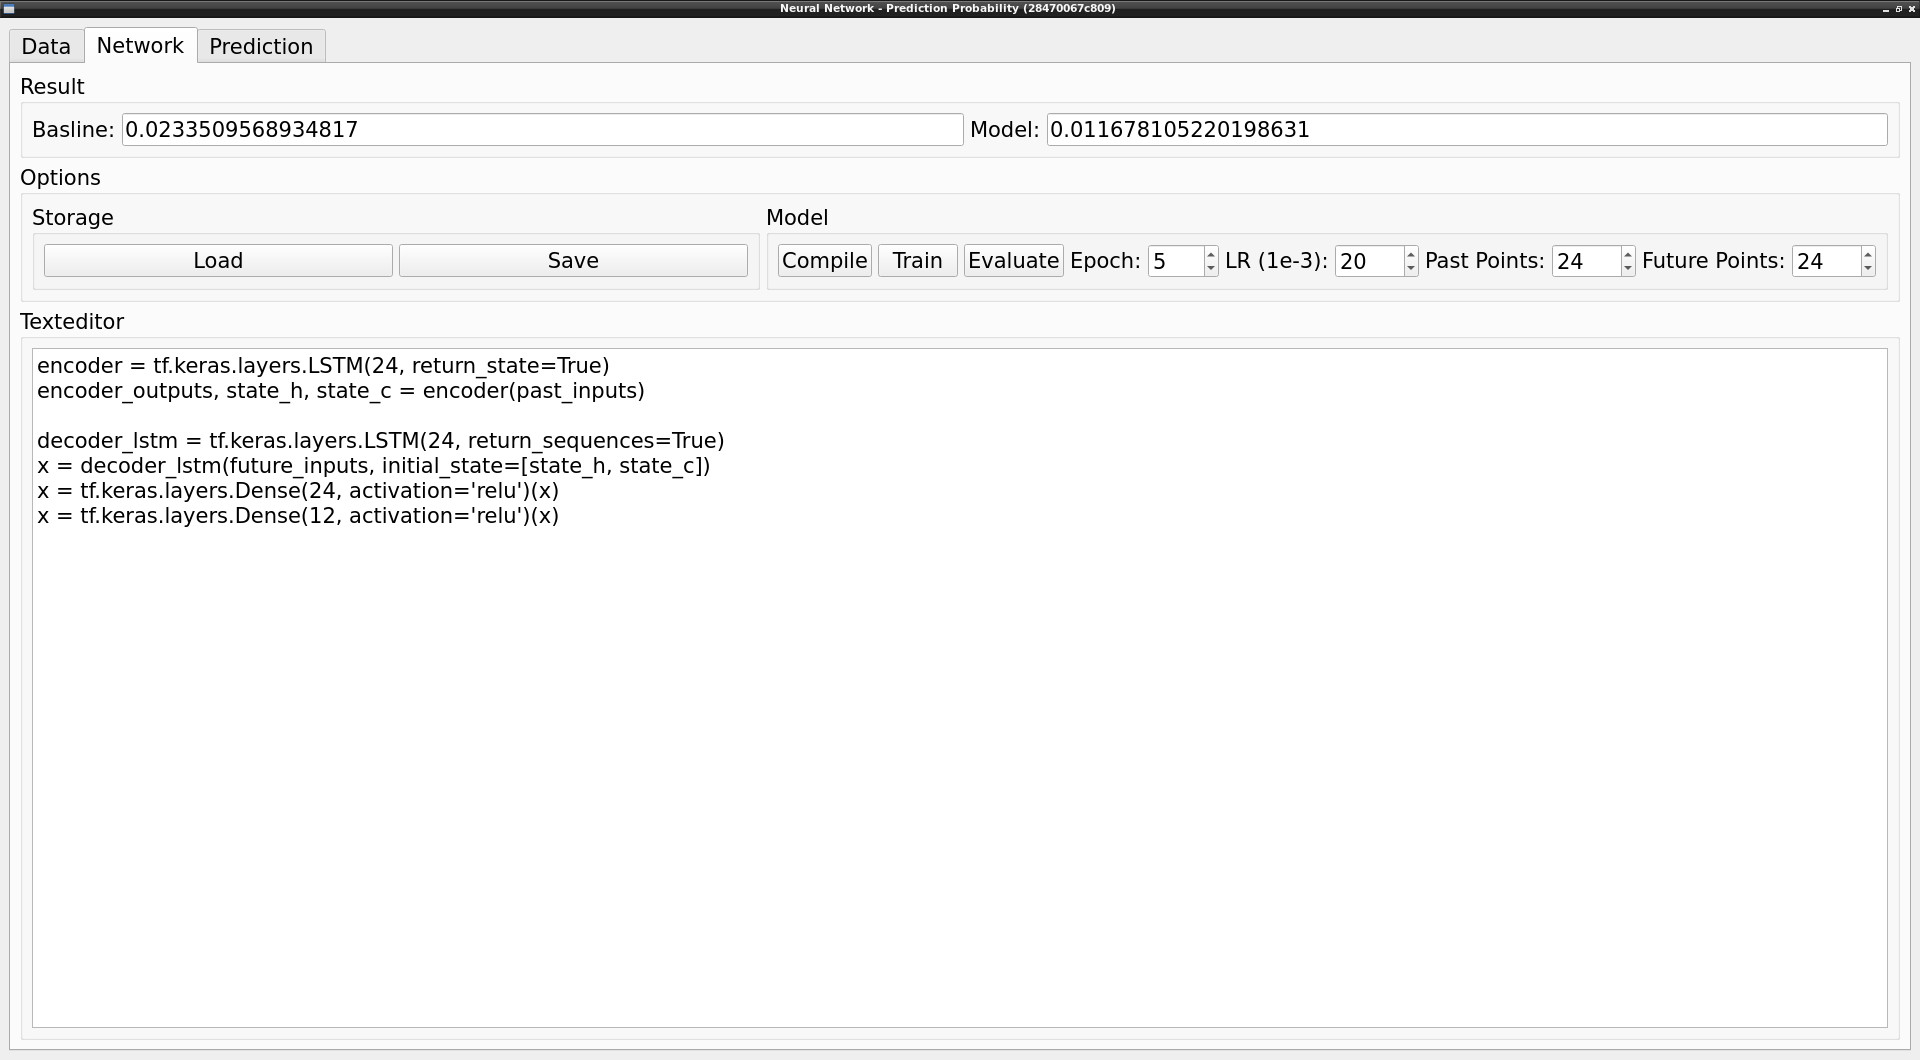
\includegraphics[width=0.9\textwidth]{./4_GUI/gui_network_tab.jpg}
		\caption{Screenshot of the network tab of the GUI. On the top are the \ac{nn} results, options and hyperparameter definitions. At the bottom a model can be defined in the texteditor.}
		\label{f:gui_network_tab}
		\end{figure}

		In case one wants to build a simple model, e.g. a \acf{fnn}, the layers can be concatenated like in the example code \ref{p:nn_example} below. If one doesn't want to use the \enquote{future\_inputs} or if they are not needed, they can plainly stay unused without negative consequences.
		
		\newpage
		\begin{lstlisting}[caption={Linear Fit}, language=python, label={p:nn_example}]
a = tf.keras.layers.Dense(4, activation='relu')
  (past_inputs)
b = tf.keras.layers.Dense(4, activation='relu')
  (future_inputs)  
x = tf.keras.layers.concatenate([a, b])
x = tf.keras.layers.Dense(4, activation='relu')(x)
		\end{lstlisting}
		
		
		\subsection{Prediction Tab}
		The prediction tab in figure \ref{f:gui_prediction_tab} follows the network tab and can be used to visualize the output of the trained network.
		
		Once the network is compiled and trained, one can verify the results on a visual basis. By clicking the \enquote{Next Example} button, the GUI randomly selects an example from the test-set and displays the ground truth in blue and the prediction value in red. Additionally the standard-deviation is shown in green with the boundaries $\pm 2\cdot\sigma$. \newline
		The plot can be magnified and also exported either as picture or as datafile with the values of the curves.
		
		\begin{figure}[htb]
		\centering
		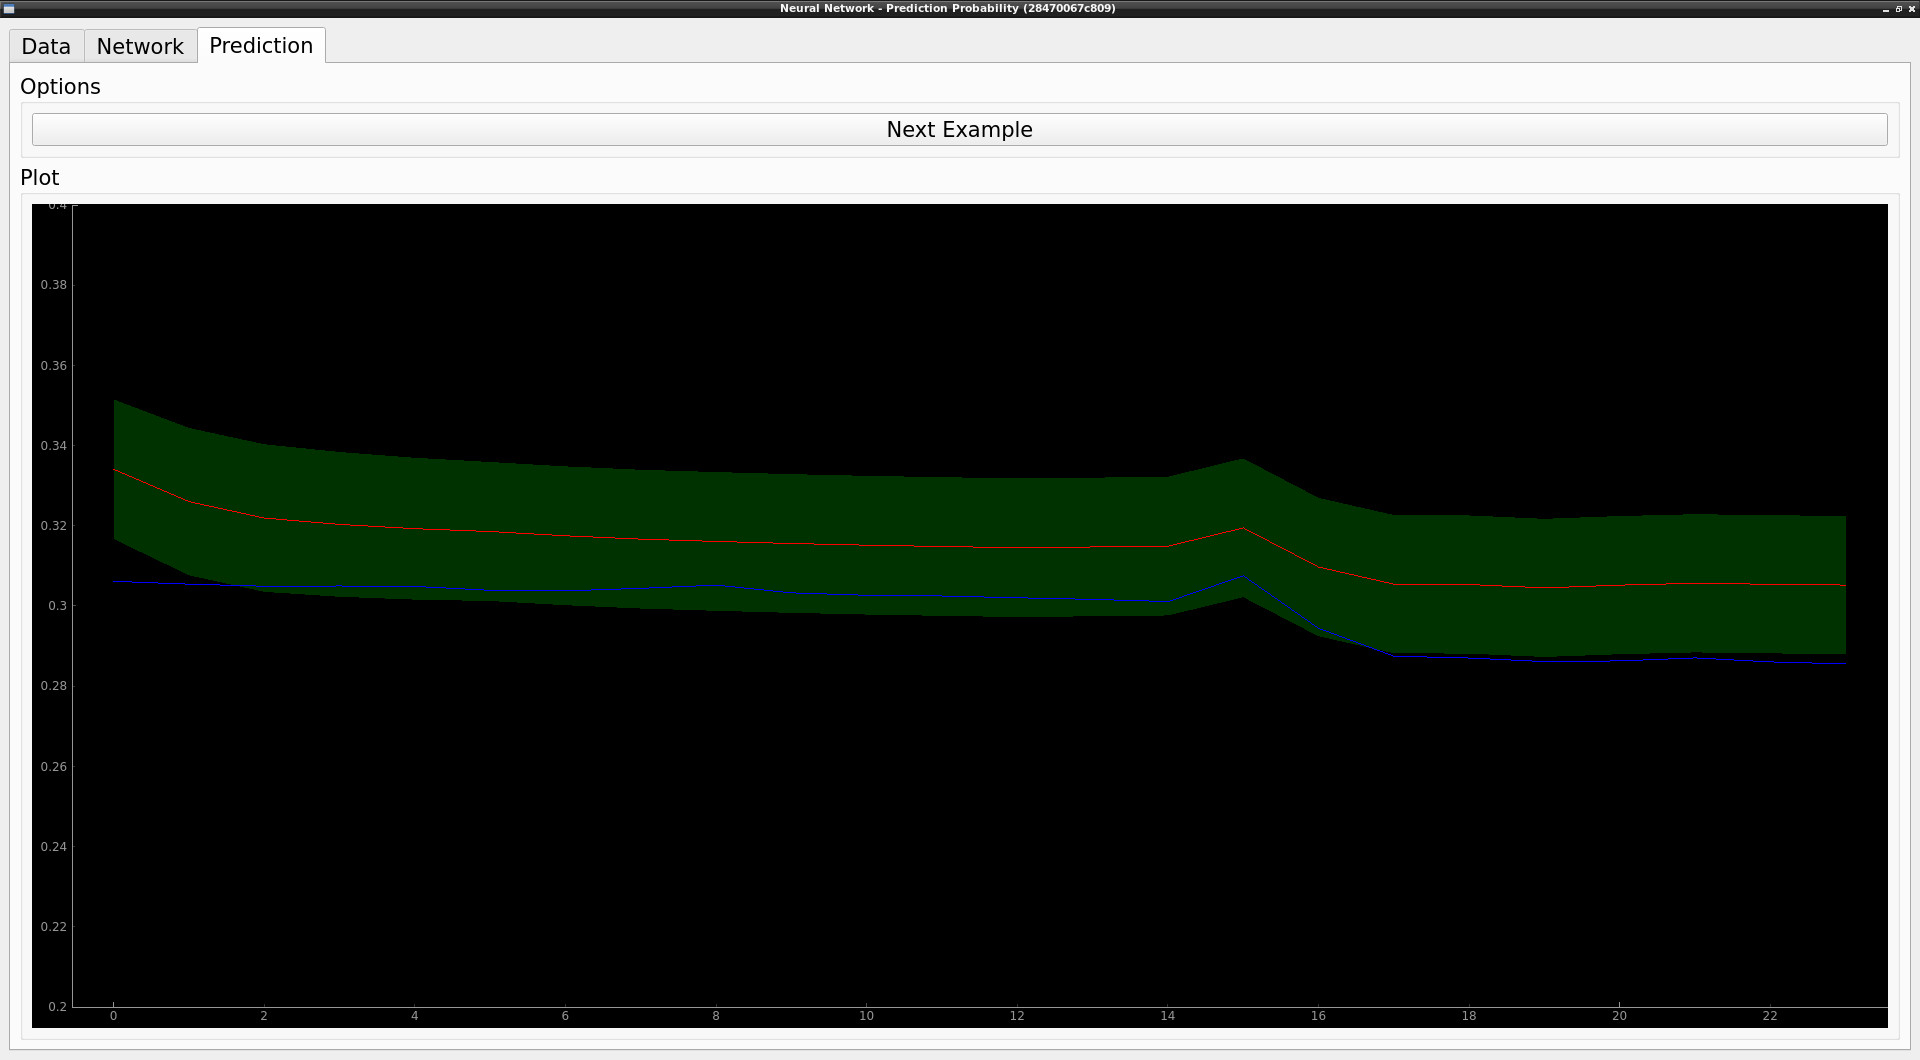
\includegraphics[width=0.9\textwidth]{./4_GUI/gui_prediction_tab.jpg}
		\caption{Screenshot of the prediction tab of the GUI. Here the prediction result with uncertainty can be visualized with random examples from the test-set.}
		\label{f:gui_prediction_tab}
		\end{figure}
